\documentclass[a4paper, 10pt, dvipdfmx]{jlreq}

\usepackage{amsmath,amsfonts,amssymb}
\usepackage{bm}
\usepackage{mathtools}
\usepackage{siunitx}
\usepackage[dvipdfmx]{graphicx}
\usepackage[dvipdfmx]{color}
\usepackage[dvipdfmx, colorlinks=true, allcolors=blue]{hyperref}
\usepackage{listings}
\usepackage{tikz}
\usepackage{physics}
\usepackage{url}

\Urlmuskip=0mu plus 10mu
\allowdisplaybreaks[4]
\frenchspacing
\definecolor{OliveGreen}{rgb}{0.0,0.6,0.0}
\definecolor{Orenge}{rgb}{0.89,0.55,0}
\definecolor{SkyBlue}{rgb}{0.28, 0.28, 0.95}
\lstset{
  language={c++},
  basicstyle={\ttfamily},
  identifierstyle={\small},
  ndkeywordstyle={\small},
  frame=single,
  breaklines=true,
  numbers=left,
  xrightmargin=0zw,
  xleftmargin=3zw,
  numberstyle={\scriptsize},
  lineskip=-0.9ex,
  keywordstyle={\small\bfseries\color{SkyBlue}},  
  commentstyle={\color{OliveGreen}}, 
  stringstyle={\small\ttfamily\color{Orenge}}    
}

\begin{document}

\title{2023年度 大問1}
\author{hari64boli64 (hari64boli64@gmail.com)}
\date{\today}
\maketitle

\section{問題}

\begin{align*}
  f(A,B)=\log{
  \frac{1}{m}\sum_{i=1}^{m}{
  \frac{1}{\frac{1}{n}\sum_{j=1}^{n}{\exp(-|a_i-b_j|)}}}
  }
\end{align*}

\section{解答}

\subsection*{(1)}

\begin{align*}
              & -|a_i-b_j| \leq 0                                                                       \\
  \Rightarrow & \frac{1}{n}\sum_{j=1}^{n}{\exp(-|a_i-b_j|)} \leq 1                                      \\
  \Rightarrow & \frac{1}{m}\sum_{i=1}^{m}{\frac{1}{\frac{1}{n}\sum_{j=1}^{n}{\exp(-|a_i-b_j|)}}} \geq 1 \\
  \Rightarrow & f(A,B) \geq 0
\end{align*}

等号成立条件は、上の式変形より、$\forall \; i,j, \; a_i=b_j$である。

\subsection*{(2)}

定義に従って示せばよい(変則的だが、分かりやすさの為、左向きの矢印を使用する)。

\begin{align*}
             & f(A,C) \leq f(A,B)+f(B,C)                                                                                                                                                                                                                                    \\
  \Leftarrow & \frac{1}{m}\sum_{i=1}^{m}{\frac{1}{\frac{1}{l}\sum_{k=1}^{l}\exp(-|a_i-c_k|)}} \leq \qty(\frac{1}{m}\sum_{i=1}^{m}{\frac{1}{\frac{1}{n}\sum_{j=1}^{n}\exp(-|a_i-b_j|)}})\qty(\frac{1}{n}\sum_{j=1}^{n}{\frac{1}{\frac{1}{l}\sum_{k=1}^{l}\exp(-|b_j-c_k|)}}) \\
  \Leftarrow & \sum_{k=1}^{l}\exp(-|a_i-c_k|) \geq \frac{\sum_{j=1}^{n}\exp(-|a_i-b_j|)}{\sum_{j=1}^{n}{\frac{1}{\sum_{k=1}^{l}\exp(-|b_j-c_k|)}}}                                                                                                                          \\
  \Leftarrow & \sum_{j=1}^{n}{\frac{\sum_{k=1}^{l}\exp(-|a_i-c_k|)}{\sum_{k=1}^{l}\exp(-|b_j-c_k|)}} \geq \sum_{j=1}^{n}\exp(-|a_i-b_j|)                                                                                                                                    \\
  \Leftarrow & \sum_{k=1}^{l}\exp(-|a_i-c_k|) \geq \exp(-|a_i-b_j|)\qty(\sum_{k=1}^{l}\exp(-|b_j-c_k|))                                                                                                                                                                     \\
  \Leftarrow & \exp(-|a_i-c_k|) \geq \exp(-|a_i-b_j|)\exp(-|b_j-c_k|)                                                                                                                                                                                                       \\
  \Leftarrow & |a_i-c_k| \leq |a_i-b_j|+|b_j-c_k|                                                                                                                                                                                                                           \\
\end{align*}

最後の不等式は、三角不等式より成立する。

以上より、$f(A,C) \leq f(A,B)+f(B,C)$が示された。

\subsection*{(3)}

区分求積法そのままなので、
\begin{align*}
  h(z)=\int_0^1{\exp(-|z-x|)}\dd{x}
\end{align*}
である。

よって、
\begin{align*}
  h(z)=
  \begin{cases}
    e^{-z}(e-1) \; (1 \leq z)       \\
    2-e^{-z}+e^{z-1} \; (0 < z < 1) \\
    e^{z}(1-e^{-1}) \; (z \leq 0)
  \end{cases}
\end{align*}
となる。

\begin{figure}[htbp]
  \begin{center}
    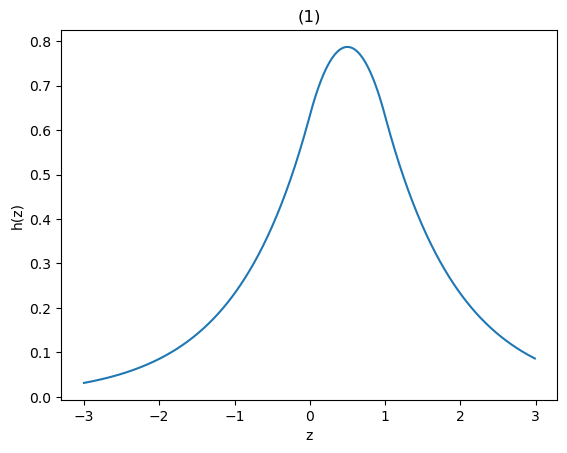
\includegraphics[width=0.5\columnwidth]{1.png}
    \caption{$h(z)$のグラフ}
    \label{fig:1}
  \end{center}
\end{figure}

\subsection*{(4)}

$h(z)$は$1/2$を中心とする対称関数であり、
微分などを計算すると、図\ref{fig:1}のようになる。

よって、
あまり厳密な議論ではないが、
区間幅1の$h(z)$の最も大きな部分は$s=0$の時に成立する。
(しかし、これは厳密に行う事も出来るはず)

以上より、$s=0$が答え。

実際、これが正しいことは、図\ref{fig:4}より分かる。

\begin{figure}[htbp]
  \begin{center}
    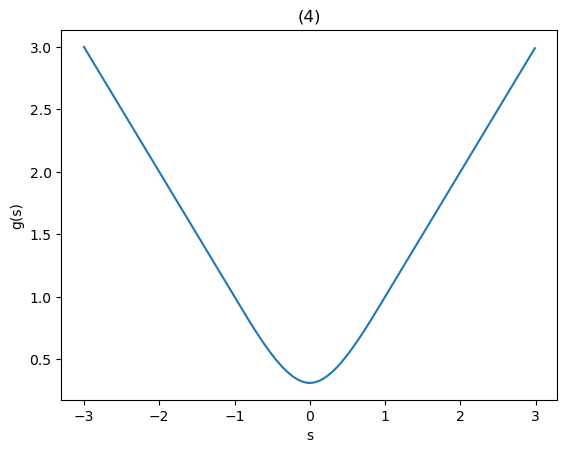
\includegraphics[width=0.5\columnwidth]{4.png}
    \caption{$g(s)$のグラフ}
    \label{fig:4}
  \end{center}
\end{figure}

\newpage

\section*{おまけ}

\lstinputlisting[caption=1,label=code:1,language=Python]{1.py}

\end{document}
